\documentclass[aps,prd,reprint,onecolumn,notitlepage,nofootinbib]{revtex4-2} % chktex 8

\usepackage[T1]{fontenc}
\usepackage{lmodern}
\usepackage{amsmath,amssymb}
\usepackage{bm}
\usepackage{booktabs}
\usepackage{graphicx}
\usepackage{microtype}
\usepackage{url}
\usepackage{hyperref}

\InputIfFileExists{sim_results.tex}{}{%
  \providecommand{\SimOutputBranch}{(26, 8, 312)}
  \providecommand{\SimOutputCanonicalBranch}{(26, 8, 312)}
  \providecommand{\SimOutputLeptonLift}{6}
  \providecommand{\SimOutputQuarkLift}{13}
  \providecommand{\SimOutputDarkResidual}{2.300805139659}
  \providecommand{\SimOutputDarkLedger}{3.300805139659}
  \providecommand{\SimOutputDarkCompleted}{3.300805139659}
  \providecommand{\SimOutputEntropyDebt}{0.137533547486}
  \providecommand{\SimOutputWarpVelocity}{1.071186351}
  \providecommand{\SimOutputPowerReq}{142.08}
  \providecommand{\SimOutputOperationalPowerMW}{142.08}
  \providecommand{\SimOutputPowerScaleRadius}{1.465189552753\times{}10^{-20}}
  \providecommand{\SimOutputSaturatedBitBudget}{3.312593327986\times{}10^{122}}
  \providecommand{\SimOutputLocalMemoryBits}{1.202481\times{}10^{72}}
  \providecommand{\SimOutputShiftFieldFormula}{\beta_x(\mathbf{x}) = -c \,e^{\Delta_{\mathrm{mod}}/2} f_{\text{SHBT}}(\mathbf{x}, \theta)}
  \providecommand{\SimOutputBoundaryPartition}{0.00342010966891}
  \providecommand{\SimOutputShannonEntropy}{0.999490161461}
  \providecommand{\SimOutputPhaseTheta}{0.421}
  \providecommand{\SimOutputFramingDefect}{0.000000000000}
  \providecommand{\SimOutputClosureNorm}{0}
  \providecommand{\SimOutputBoundaryNormError}{0}
  \providecommand{\SimOutputUnitarityError}{4.587893\times{}10^{-16}}
  \providecommand{\SimOutputPopulationShift}{0.263689500253}
  \providecommand{\SimOutputMetricDetMin}{1}
  \providecommand{\SimOutputMetricEigenMin}{0.358567865584}
  \providecommand{\SimOutputObserverMetricError}{0}
  \providecommand{\SimOutputAccelerationNorm}{0}
  \providecommand{\SimOutputNEC}{-1.495110\times{}10^{6}}
  \providecommand{\SimOutputWEC}{-8.772117\times{}10^{5}}
  \providecommand{\SimOutputSteadyStateEntropyDebt}{0.137533547486}
  \providecommand{\SimOutputMaximumHoldTimeS}{\infty}
}

\InputIfFileExists{cad_sim_results.tex}{}{%
  \providecommand{\CADCanonicalBranch}{(26, 8, 312)}
  \providecommand{\CADFramingDefect}{0.000000000000}
  \providecommand{\CADUnitarityResidual}{2.220446049250e-16}
  \providecommand{\CADPhaseJitterOk}{true}
  \providecommand{\CADThermalDecoherenceOk}{true}
  \providecommand{\CADIntegerLockOk}{true}
  \providecommand{\CADStinespringRatio}{0.697043612789}
  \providecommand{\CADDeltaMod}{0.137533547486}
  \providecommand{\CADMetricDeterminant}{-1.000000000000}
  \providecommand{\CADRadius}{10.0}
  \providecommand{\CADPhase}{0.421000}
  \providecommand{\CADEmitterThetaK}{0.285186702072}
  \providecommand{\CADEmitterVRF}{9.443489112879e-01}
}

\begin{document}
\title{Phase-Locked Boundary Entanglement Engineering and Holographic Warp Metrics: A Static Holographic Boundary Theory Investigation}
\date{\today}
\maketitle

% chktex-file 35
% chktex-file 3
\section{Introduction and holographic framework}\label{sec:introduction}

Metric engineering in classical general relativity is an inverse problem.  One first specifies a target Lorentzian geometry \(g_{\mu\nu}^{\mathrm{target}}\), computes its Einstein tensor, and then infers the stress-energy tensor required to sustain it:
\begin{equation}
  T_{\mu\nu}^{\mathrm{req}}
  =
  \frac{1}{8\pi G_N}
  \left(
    G_{\mu\nu}[g^{\mathrm{target}}]
    +\Lambda g_{\mu\nu}^{\mathrm{target}}
  \right).
  \label{eq:gr-inverse-problem}
\end{equation}
For an Alcubierre-type longitudinal shift, the wall gradients of the prescribed shape function generate regions in which the Eulerian energy density is negative,
\begin{equation}
  \rho_{\mathrm{GR}}
  =
  T_{\mu\nu}^{\mathrm{req}}n^\mu n^\nu
  <0,
  \qquad\text{and hence}\qquad
  T_{00}<0
  \quad\text{in part of the wall}.
  \label{eq:classical-negative-energy}
\end{equation}
The obstruction is therefore not merely technological: the target metric is supported by a bulk source that violates the weak energy condition and, for appropriate null directions, the null energy condition.

Static Holographic Boundary Theory (SHBT) changes the control problem.  The independent data are assigned to a static boundary conformal register, while the bulk metric is treated as a downstream projection of boundary loading, Shannon entanglement, and holographic resolution flow.  The foundational construction and its numerical implementation are established in the primary repository
\url{https://github.com/sys1own/shbt-precision.git}.  In the extension studied here, no negative-energy bulk source is inserted into Eq.~\eqref{eq:gr-inverse-problem}.  Instead, a unitary character excitation redistributes boundary entanglement and the resulting directional entropy shear is mapped into a bulk shift component.  The operational distinction is
\begin{equation}
  \text{classical GR:}\quad
  g_{\mu\nu}^{\mathrm{target}}
  \longrightarrow T_{\mu\nu}^{\mathrm{req}},
  \qquad
  \text{SHBT:}\quad
  \rho_{\partial}
  \longrightarrow \rho_E
  \longrightarrow \Phi_s^{(x)}
  \longrightarrow g_{\mu\nu}.
  \label{eq:bulk-versus-boundary-control}
\end{equation}
Thus \emph{matter-free} refers specifically to the absence of an imposed exotic bulk source.  Control hardware and positive boundary bookkeeping costs remain part of the physical accounting.

\subsection{Canonical anomaly-free branch}

The visible boundary theory is the affine product
\begin{equation}
  \mathcal{A}_{\mathrm{vis}}
  =
  \mathrm{SU}(2)_{k_\ell}
  \times
  \mathrm{SU}(3)_{k_q},
  \qquad
  \mathfrak{b}_*
  =
  (k_\ell,k_q,K)
  =
  (26,8,312)
  =
  \SimOutputBranch,
  \label{eq:canonical-anomaly-free-branch}
\end{equation}
embedded in the parent completion \(\mathrm{SO}(10)_K\).  The corresponding center lifts are
\begin{equation}
  \begin{aligned}
  I_\ell^*
  &=
  \frac{K}{2k_\ell}
  =
  \frac{312}{52}
  =
  6,
  \\
  I_q^*
  &=
  \frac{K}{3k_q}
  =
  \frac{312}{24}
  =
  13.
  \end{aligned}
  \label{eq:integer-center-lifts}
\end{equation}
For \(\|x\|_{\mathbb Z}\equiv\min_{n\in\mathbb Z}|x-n|\), the scalar framing defect is
\begin{equation}
  \Delta_{\mathrm{fr}}(\mathfrak b)
  =
  \max\left\{
    \left\|\frac{K}{2k_\ell}\right\|_{\mathbb Z},
    \left\|\frac{K}{3k_q}\right\|_{\mathbb Z}
  \right\}.
  \label{eq:framing-defect-general}
\end{equation}
Equations~\eqref{eq:canonical-anomaly-free-branch} and~\eqref{eq:integer-center-lifts} imply
\begin{equation}
  \Delta_{\mathrm{fr}}(\mathfrak b_*)
  =
  \max\{\|6\|_{\mathbb Z},\|13\|_{\mathbb Z}\}
  =
  0.
  \label{eq:zero-framing-defect}
\end{equation}

The framing condition is not an optional numerical tolerance.  Within the SHBT closure ansatz, the scalar obstruction has the unique metric-proportional bulk continuation
\begin{equation}
  \mathcal{E}_{\mu\nu}
  =
  \mathcal{Q}_{\mathrm{fr}}
  \Delta_{\mathrm{fr}}
  g_{\mu\nu},
  \label{eq:weyl-closure-tensor}
\end{equation}
where \(\mathcal{Q}_{\mathrm{fr}}\) is the framing-response coefficient.  Therefore
\begin{equation}
  \begin{aligned}
  \Delta_{\mathrm{fr}}=0
  &\quad\Longrightarrow\quad
  \mathcal{E}_{\mu\nu}=0,
  \\
  \|\mathcal E\|_g
  &=
  |\mathcal Q_{\mathrm{fr}}|
  |\Delta_{\mathrm{fr}}|
  \|g\|_g
  =
  0.
  \end{aligned}
  \label{eq:closure-tensor-vanishes}
\end{equation}
Any intervention that changes the affine levels may reopen \(\Delta_{\mathrm{fr}}\), inject a framing-sourced Weyl term, and invalidate the closed boundary-to-bulk projection.  Admissible controls must consequently act inside the fixed nine-dimensional visible block and preserve the branch \(\mathfrak b_*\) exactly.

\subsection{Holographic control variables}

The completed dark ledger and its dimensionless modular debt are
\begin{equation}
  \begin{aligned}
  c_{\mathrm{dark}}^{\mathrm{comp}}
  &=
  \frac{1197103}{362670}
  =
  \SimOutputDarkLedger,
  \\
  \Delta_{\mathrm{mod}}
  &=
  \frac{c_{\mathrm{dark}}^{\mathrm{comp}}}{24}
  =
  \frac{1197103}{8704080}
  =
  \SimOutputEntropyDebt.
  \end{aligned}
  \label{eq:intro-dark-ledger}
\end{equation}
The extension assigns the corresponding kinematic scale
\begin{equation}
  v_{\mathrm{eff}}
  =
  c\exp\left(\frac{\Delta_{\mathrm{mod}}}{2}\right),
  \qquad
  \frac{v_{\mathrm{eff}}}{c}
  =
  \SimOutputWarpVelocity.
  \label{eq:intro-effective-velocity}
\end{equation}
These definitions do not by themselves establish a realizable propulsion system.  They specify a closed mathematical model whose consistency can be tested by modular invariance, unitary excitation, framing closure, metric nonsingularity, and positivity of the Euclidean Gram representative.  Sections~\ref{sec:boundary-register} and~\ref{sec:shift-derivation} construct those ingredients explicitly and distinguish the positive projection metric from the Lorentzian spacetime metric into which the shift is embedded.
% chktex-file 3
% chktex-file 8
% chktex-file 35
\section{Boundary register architecture and character excitations}\label{sec:boundary-register}

\subsection{Nine-component visible modular register}

The visible coordinate set is the Cartesian product of three \(\mathrm{SU}(2)_{26}\) charge labels and three low \(\mathrm{SU}(3)_8\) weights:
\begin{equation}
  \mathcal C
  =
  \left\{
    c_{ij}=(i,j)
    \,\middle|\,
    q_i\in(22,23,26),
    \;
    w_j\in\bigl((0,0),(1,0),(0,1)\bigr)
  \right\}.
  \label{eq:visible-register-set}
\end{equation}
The associated visible Hilbert space and coordinate projectors are
\begin{equation}
  \mathcal H_{\mathrm{vis}}
  =
  \operatorname{span}
  \left\{
    |q_i,w_j\rangle
  \right\}_{i,j=0}^{2},
  \qquad
  \Pi_{ij}
  =
  |q_i,w_j\rangle
  \langle q_i,w_j|.
  \label{eq:visible-hilbert-space}
\end{equation}
Consequently \(\dim\mathcal H_{\mathrm{vis}}=9\), and any visible density matrix is represented by a \(9\times9\) positive semidefinite matrix of unit trace.

The modular loading is obtained from the visible blocks of the \(\mathrm{SU}(2)_{26}\) and \(\mathrm{SU}(3)_8\) modular \(S\) matrices.  With the baseline charge embedding used on both \(\mathrm{SU}(2)\) axes, the raw loading is
\begin{equation}
  \widetilde{\rho}_{\bar E}(i,j)
  =
  \left|
    S^{\mathrm{SU}(2)_{26}}_{q_i,q_j}
  \right|^2
  \left|
    S^{\mathrm{SU}(3)_8}_{w_i,w_j}
  \right|^2.
  \label{eq:raw-visible-register-loading}
\end{equation}
The \(\mathrm{SU}(2)\) kernel is
\begin{equation}
  S^{\mathrm{SU}(2)_{26}}_{ab}
  =
  \sqrt{\frac{2}{28}}
  \sin\left[
    \frac{\pi(a+1)(b+1)}{28}
  \right].
  \label{eq:su2-modular-kernel-full}
\end{equation}
For \(\lambda=(p,q)\), define the three-vector and Weyl vector
\begin{equation}
  v(p,q)
  =
  \frac{1}{3}
  \left(
    2p+q,\,
    q-p,\,
    -2p-q
  \right),
  \qquad
  \varrho=v(1,1).
  \label{eq:su3-weight-vector}
\end{equation}
The corresponding \(\mathrm{SU}(3)_8\) Weyl-sum kernel is
\begin{equation}
  S^{\mathrm{SU}(3)_8}_{\lambda\mu}
  =
  -\frac{i}{11\sqrt{3}}
  \sum_{\sigma\in S_3}
  \operatorname{sgn}(\sigma)
  \exp\left[
    -\frac{2\pi i}{11}
    \left(
      \sigma[v(\lambda)+\varrho],
      v(\mu)+\varrho
    \right)
  \right].
  \label{eq:su3-modular-kernel-full}
\end{equation}

The boundary normalization and normalized visible loading density are
\begin{equation}
  Z_{\partial}
  =
  \sum_{i,j=0}^{2}
  \widetilde{\rho}_{\bar E}(i,j),
  \qquad
  \rho_{\bar E}(i,j)
  =
  \frac{\widetilde{\rho}_{\bar E}(i,j)}
  {Z_{\partial}},
  \qquad
  \sum_{i,j=0}^{2}\rho_{\bar E}(i,j)=1.
  \label{eq:normalized-visible-loading}
\end{equation}
The executable prototype evaluates
\begin{equation}
  Z_{\partial}
  =
  \SimOutputBoundaryPartition,
  \qquad
  \left|
    \sum_{i,j}\rho_{\bar E}(i,j)-1
  \right|
  =
  \SimOutputBoundaryNormError.
  \label{eq:register-numerical-normalization}
\end{equation}
The local Shannon contributions, total visible entropy, and normalized entanglement density are
\begin{equation}
  s_{ij}
  =
  -\rho_{\bar E}(i,j)
  \ln\rho_{\bar E}(i,j),
  \qquad
  S_E
  =
  \sum_{i,j=0}^{2}s_{ij},
  \qquad
  \rho_E(i,j)
  =
  \frac{s_{ij}}{S_E}.
  \label{eq:visible-shannon-density}
\end{equation}
Thus \(\sum_{i,j}\rho_E(i,j)=1\), while the computed baseline entropy is
\begin{equation}
  S_E
  =
  \SimOutputShannonEntropy.
  \label{eq:baseline-shannon-entropy}
\end{equation}

\subsection{Phase-locked character excitation}

Write each \(\mathrm{SU}(3)\) weight as \(w_j=(p_j,r_j)\) and define its scalar grade
\begin{equation}
  \nu(w_j)
  =
  p_j+r_j.
  \label{eq:su3-scalar-grade}
\end{equation}
To preserve the compact notation requested for character phases, we use \(q_i+w_j\) as shorthand for \(q_i+\nu(w_j)\).  The explicit character modulation factor is therefore
\begin{equation}
  \chi_{ij}^{\mathrm{char}}(\theta)
  =
  e^{i\theta(q_i+w_j)}
  \equiv
  \exp\left\{
    i\theta
    \left[
      q_i+\nu(w_j)
    \right]
  \right\}.
  \label{eq:explicit-character-phase}
\end{equation}
The conformal dimensions and visible central charge are
\begin{equation}
  h_{ij}
  =
  \frac{q_i(q_i+2)}{4(26+2)}
  +
  \frac{p_j^2+r_j^2+p_j r_j+3p_j+3r_j}
  {3(8+3)},
  \qquad
  c_{\mathrm{vis}}
  =
  \frac{39}{14}
  +
  \frac{64}{11}
  =
  \frac{1325}{154}.
  \label{eq:visible-conformal-data}
\end{equation}
The diagonal phase-locking operator combines the character phase with the modular \(T\)-phase:
\begin{equation}
  M_{\mathrm{phase}}(\theta)
  =
  \sum_{i,j=0}^{2}
  \exp\left\{
    i\theta[q_i+\nu(w_j)]
    +
    2\pi i\theta
    \left(
      h_{ij}-\frac{c_{\mathrm{vis}}}{24}
    \right)
  \right\}
  \Pi_{ij}.
  \label{eq:full-phase-locking-operator}
\end{equation}
Let \(G_x=G_x^\dagger\) be the directional generator that couples adjacent charge sectors at fixed \(\mathrm{SU}(3)\) weight.  The unitary excitation operator is
\begin{equation}
  \widehat{\mathcal O}_{\mathrm{excitation}}(\theta)
  =
  e^{-i\theta G_x}
  M_{\mathrm{phase}}(\theta),
  \qquad
  0\leq\theta<2\pi.
  \label{eq:unitary-excitation-operator}
\end{equation}
Because \(G_x\) is Hermitian and every diagonal phase has unit modulus,
\begin{equation}
  \widehat{\mathcal O}_{\mathrm{excitation}}^\dagger(\theta)
  \widehat{\mathcal O}_{\mathrm{excitation}}(\theta)
  =
  M_{\mathrm{phase}}^\dagger
  e^{i\theta G_x}
  e^{-i\theta G_x}
  M_{\mathrm{phase}}
  =
  \mathbb I_9.
  \label{eq:excitation-unitarity-proof}
\end{equation}
The numerical infinity-norm residual is
\begin{equation}
  \left\|
    \widehat{\mathcal O}_{\mathrm{excitation}}^\dagger
    \widehat{\mathcal O}_{\mathrm{excitation}}
    -
    \mathbb I_9
  \right\|_{\infty}
  =
  \SimOutputUnitarityError.
  \label{eq:excitation-unitarity-residual}
\end{equation}

For a baseline state \(\rho_\partial\), the excited state and observable coordinate probabilities are
\begin{equation}
  \rho_\partial^{(\theta)}
  =
  \frac{
    \widehat{\mathcal O}_{\mathrm{excitation}}(\theta)
    \rho_\partial
    \widehat{\mathcal O}_{\mathrm{excitation}}^\dagger(\theta)
  }{
    \operatorname{Tr}\left[
      \widehat{\mathcal O}_{\mathrm{excitation}}(\theta)
      \rho_\partial
      \widehat{\mathcal O}_{\mathrm{excitation}}^\dagger(\theta)
    \right]
  },
  \qquad
  \rho_{\bar E}^{(\theta)}(i,j)
  =
  \operatorname{Tr}
  \left[
    \Pi_{ij}\rho_\partial^{(\theta)}
  \right].
  \label{eq:excited-register-state}
\end{equation}
Its normalized directional Shannon density is
\begin{equation}
  \rho_E^{(\theta)}(i,j)
  =
  \frac{
    -\rho_{\bar E}^{(\theta)}(i,j)
    \ln\rho_{\bar E}^{(\theta)}(i,j)
  }{
    -\sum_{a,b}
    \rho_{\bar E}^{(\theta)}(a,b)
    \ln\rho_{\bar E}^{(\theta)}(a,b)
  }.
  \label{eq:excited-shannon-density}
\end{equation}
At the benchmark angle \(\theta=\SimOutputPhaseTheta\), the prototype obtains the nonzero population displacement
\begin{equation}
  \sum_{i,j}
  \left|
    \rho_{\bar E}^{(\theta)}(i,j)
    -
    \rho_{\bar E}(i,j)
  \right|
  =
  \SimOutputPopulationShift.
  \label{eq:population-displacement}
\end{equation}

\begin{figure}
  \centering
  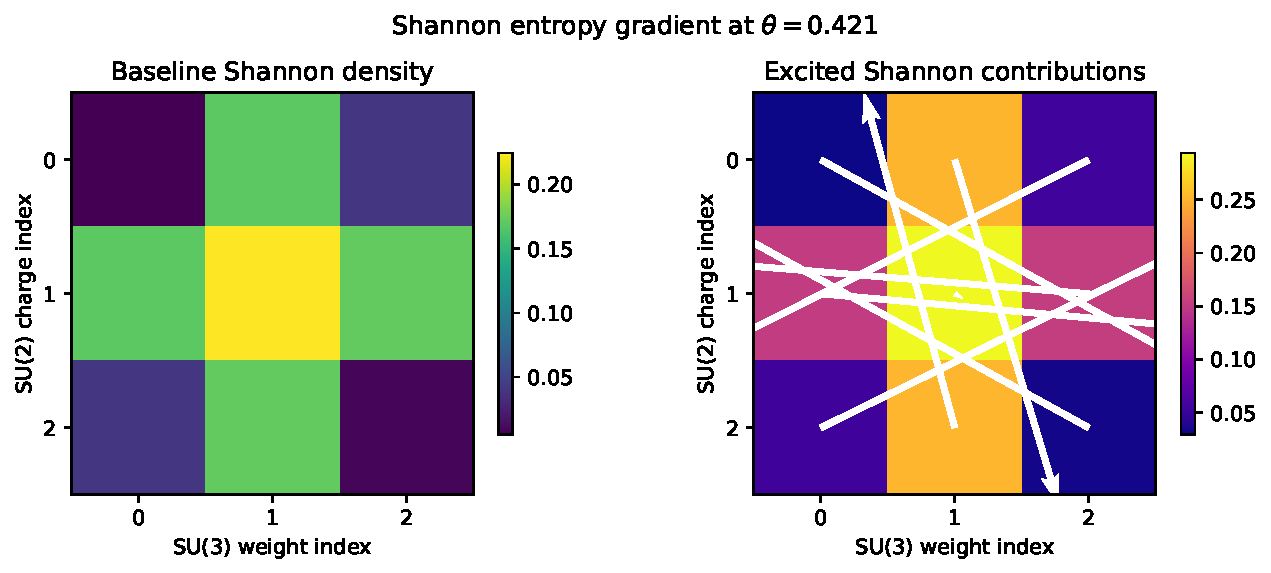
\includegraphics[width=0.86\columnwidth]{figures/entropy_gradient.pdf}
  \caption{Baseline and phase-locked Shannon contributions at
  \(\theta=\SimOutputPhaseTheta\).  The arrows display the discrete gradient
  of the excited entropy contribution.}\label{fig:entropy-gradient}
\end{figure}

\subsection{Directional entropy shear}

Order the nine coordinates by a fixed sequence
\begin{equation}
  \sigma
  =
  (c_1,c_2,\ldots,c_9),
  \qquad
  c_m\in\mathcal C,
  \label{eq:ordered-visible-sequence}
\end{equation}
and fold that sequence onto the prime skeleton
\begin{equation}
  (p_0,p_1,p_2,p_3,p_4)
  =
  (2,3,5,7,11),
  \qquad
  x_r^{(p)}
  =
  \ln p_r.
  \label{eq:prime-skeleton}
\end{equation}
Let \(\chi_m^{(x)}\) be the signed longitudinal character of coordinate \(c_m\), normalized so that \(|\chi_m^{(x)}|\leq1\).  At holographic resolution \(\tau\), the directional prime-load vector is
\begin{equation}
  \ell_r^{(x)}(\theta,\boldsymbol{x};\tau)
  =
  \frac{1}{1+\tau}
  \sum_{m=1}^{9}
  \rho_E^{(\theta)}(c_m)
  \left[
    1+
    \frac{x}{R_{\mathrm{bubble}}}
    \chi_m^{(x)}
  \right]
  \mathbb I_{\{m-1\equiv r\;(\mathrm{mod}\;5)\}},
  \qquad
  r=0,\ldots,4.
  \label{eq:directional-prime-load}
\end{equation}
The longitudinal Euler flux on the four prime intervals is then
\begin{equation}
  \Phi_s^{(x)}(\theta,\boldsymbol{x};\tau)
  =
  \frac{
    \ell_{s+1}^{(x)}(\theta,\boldsymbol{x};\tau)
    -
    \ell_s^{(x)}(\theta,\boldsymbol{x};\tau)
  }{
    \ln(p_{s+1}/p_s)
  },
  \qquad
  s=0,1,2,3.
  \label{eq:directional-entropy-shear}
\end{equation}
This quantity is the discrete boundary derivative that carries directional information into the bulk projector.  It vanishes for a load vector that is constant on the logarithmic prime lattice and changes sign under reversal of the longitudinal orientation.

Finally, the excitation remains on the fixed branch,
\begin{equation}
  \widehat{\mathcal O}_{\mathrm{excitation}}(\theta):
  \mathcal H_{\mathrm{vis}}(\mathfrak b_*)
  \longrightarrow
  \mathcal H_{\mathrm{vis}}(\mathfrak b_*),
  \qquad
  \delta k_\ell
  =
  \delta k_q
  =
  \delta K
  =
  0.
  \label{eq:branch-preserving-excitation}
\end{equation}
Since \(\Delta_{\mathrm{fr}}\) depends only on these discrete levels,
\begin{equation}
  \Delta_{\mathrm{fr}}(\theta)
  =
  \Delta_{\mathrm{fr}}(\mathfrak b_*)
  =
  0,
  \qquad
  \mathcal E_{\mu\nu}(\theta)
  =
  0
  \quad
  \text{for every admissible }\theta.
  \label{eq:framing-preserved-under-excitation}
\end{equation}
% chktex-file 3
% chktex-file 8
% chktex-file 35
\section{First-principles shift-field derivation}\label{sec:shift-derivation}

\subsection{Constrained boundary action}

Let \(\Sigma_\partial\) denote the two-dimensional conformal boundary with induced metric \(\gamma_{ab}\).  The phase-locked state is
\begin{equation}
  \rho_\partial^{(\theta)}
  =
  \widehat{\mathcal O}_{\mathrm{excitation}}(\theta)
  \rho_\partial
  \widehat{\mathcal O}_{\mathrm{excitation}}^\dagger(\theta),
  \qquad
  \operatorname{Tr}\rho_\partial^{(\theta)}=1.
  \label{eq:section3-excited-state}
\end{equation}
The on-shell boundary condition stated in \(warp2.txt\) is the constrained stationarity requirement
\begin{equation}
  \delta\mathcal S_{\mathrm{CFT}}
  =
  \int_{\Sigma_\partial}
  d^2y\sqrt{-\gamma}
  \left[
    \frac{\delta\mathcal L_{\mathrm{CFT}}}
    {\delta\widehat{\mathcal O}_{\mathrm{excitation}}}
    \delta\widehat{\mathcal O}_{\mathrm{excitation}}
    +
    \frac{\partial\mathcal L_{\mathrm{anomaly}}}
    {\partial\Delta_{\mathrm{fr}}}
    \delta\Delta_{\mathrm{fr}}
  \right]
  =
  0,
  \qquad
  \Delta_{\mathrm{fr}}=0.
  \label{eq:boundary-action-stationarity}
\end{equation}
To make the metric response explicit, introduce the reduced boundary-to-bulk functional
\begin{equation}
  \mathcal S_{\mathrm{red}}
  \left[
    \rho_\partial^{(\theta)},
    \beta_x,
    \lambda_{\mathrm{fr}}
  \right]
  =
  \mathcal S_{\mathrm{CFT}}
  \left[
    \rho_\partial^{(\theta)}
  \right]
  +
  \mathcal S_{\mathrm{proj}}
  +
  \mathcal S_{\mathrm{fr}},
  \label{eq:reduced-boundary-functional}
\end{equation}
where
\begin{equation}
  \mathcal S_{\mathrm{proj}}
  =
  \frac{\kappa_\beta}{2}
  \int_{\Sigma_\partial}
  d^2y\sqrt{-\gamma}
  \left[
    \beta_x(\boldsymbol{x})
    +
    v_{\mathrm{eff}}
    \mathcal A_x(\theta,\boldsymbol{x})
  \right]^2,
  \qquad
  \kappa_\beta>0,
  \label{eq:projection-action}
\end{equation}
and
\begin{equation}
  \mathcal S_{\mathrm{fr}}
  =
  \int_{\Sigma_\partial}
  d^2y\sqrt{-\gamma}\,
  \lambda_{\mathrm{fr}}(y)
  \Delta_{\mathrm{fr}}.
  \label{eq:framing-lagrange-term}
\end{equation}
The first term contains the intrinsic CFT dynamics.  The second is the minimal local, nonnegative response functional whose stationary point identifies the longitudinal ADM shift with the normalized boundary flux.  The third imposes exact framing closure.

Variation with respect to the Lagrange multiplier gives
\begin{equation}
  \frac{\delta\mathcal S_{\mathrm{red}}}
  {\delta\lambda_{\mathrm{fr}}}
  =
  \sqrt{-\gamma}
  \Delta_{\mathrm{fr}}
  =
  0,
  \qquad
  \Longrightarrow
  \qquad
  \Delta_{\mathrm{fr}}=0.
  \label{eq:framing-constraint-from-action}
\end{equation}
Because the phase-locked excitation leaves the affine levels unchanged, Eq.~\eqref{eq:framing-constraint-from-action} is compatible with Eq.~\eqref{eq:framing-preserved-under-excitation} for every admissible value of \(\theta\).

\subsection{Flux functional and Euler-Lagrange equation}

Choose fixed real interval weights \(\omega_s\), and define the unnormalized longitudinal flux functional
\begin{equation}
  \mathcal F_x(\theta,\boldsymbol{x};\tau)
  =
  \sum_{s=0}^{3}
  \omega_s
  \Phi_s^{(x)}(\theta,\boldsymbol{x};\tau).
  \label{eq:unnormalized-longitudinal-flux}
\end{equation}
Its normalization over the spatial control domain \(\Omega\) is
\begin{equation}
  \mathcal N_x(\theta;\tau)
  =
  \max_{\boldsymbol{x}'\in\Omega}
  \left|
    \mathcal F_x(\theta,\boldsymbol{x}';\tau)
  \right|.
  \label{eq:longitudinal-flux-normalization}
\end{equation}
For \(\mathcal N_x>0\), the SHBT shape functional is
\begin{equation}
  f_{\mathrm{SHBT}}(\boldsymbol{x},\theta;\tau)
  \equiv
  \mathcal A_x(\theta,\boldsymbol{x};\tau)
  =
  \frac{
    \displaystyle
    \sum_{s=0}^{3}
    \omega_s
    \frac{
      \ell_{s+1}^{(x)}(\theta,\boldsymbol{x};\tau)
      -
      \ell_s^{(x)}(\theta,\boldsymbol{x};\tau)
    }{
      \ln(p_{s+1}/p_s)
    }
  }{
    \displaystyle
    \max_{\boldsymbol{x}'\in\Omega}
    \left|
      \sum_{s=0}^{3}
      \omega_s
      \frac{
        \ell_{s+1}^{(x)}(\theta,\boldsymbol{x}';\tau)
        -
        \ell_s^{(x)}(\theta,\boldsymbol{x}';\tau)
      }{
        \ln(p_{s+1}/p_s)
      }
    \right|
  }.
  \label{eq:shbt-shape-functional}
\end{equation}
By construction,
\begin{equation}
  \left|
    f_{\mathrm{SHBT}}(\boldsymbol{x},\theta;\tau)
  \right|
  \leq1.
  \label{eq:shape-functional-bound}
\end{equation}

The first variation of Eq.~\eqref{eq:projection-action} with respect to \(\beta_x\) is
\begin{equation}
  \delta_{\beta}\mathcal S_{\mathrm{red}}
  =
  \kappa_\beta
  \int_{\Sigma_\partial}
  d^2y\sqrt{-\gamma}
  \left[
    \beta_x(\boldsymbol{x})
    +
    v_{\mathrm{eff}}
    f_{\mathrm{SHBT}}(\boldsymbol{x},\theta;\tau)
  \right]
  \delta\beta_x(\boldsymbol{x}).
  \label{eq:first-variation-beta}
\end{equation}
Since \(\delta\beta_x\) is arbitrary, stationarity requires the Euler-Lagrange equation
\begin{equation}
  \frac{\delta\mathcal S_{\mathrm{red}}}
  {\delta\beta_x(\boldsymbol{x})}
  =
  \kappa_\beta\sqrt{-\gamma}
  \left[
    \beta_x(\boldsymbol{x})
    +
    v_{\mathrm{eff}}
    f_{\mathrm{SHBT}}(\boldsymbol{x},\theta;\tau)
  \right]
  =
  0.
  \label{eq:beta-euler-lagrange-equation}
\end{equation}
The unique minimum follows from the positive second variation,
\begin{equation}
  \delta_{\beta}^{2}\mathcal S_{\mathrm{red}}
  =
  \kappa_\beta
  \int_{\Sigma_\partial}
  d^2y\sqrt{-\gamma}
  \left[
    \delta\beta_x(\boldsymbol{x})
  \right]^2
  >0
  \quad
  \text{for }
  \delta\beta_x\neq0.
  \label{eq:positive-second-variation}
\end{equation}
Therefore the stationary longitudinal shift is
\begin{equation}
  \boxed{
  \beta_x(\boldsymbol{x})
  =
  -v_{\mathrm{eff}}
  f_{\mathrm{SHBT}}(\boldsymbol{x},\theta;\tau)
  }.
  \label{eq:stationary-shift-field}
\end{equation}

The topological entropy debt fixes the velocity scale,
\begin{equation}
  \Delta_{\mathrm{mod}}
  =
  \frac{c_{\mathrm{dark}}^{\mathrm{comp}}}{24}
  =
  \frac{1197103}{8704080},
  \qquad
  v_{\mathrm{eff}}
  =
  c
  \exp\left(
    \frac{\Delta_{\mathrm{mod}}}{2}
  \right).
  \label{eq:topological-velocity-scale}
\end{equation}
Combining Eqs.~\eqref{eq:stationary-shift-field} and~\eqref{eq:topological-velocity-scale} gives the requested first-principles profile:
\begin{equation}
  \boxed{
  \beta_x(\boldsymbol{x})
  =
  -c
  \exp\left(
    \frac{\Delta_{\mathrm{mod}}}{2}
  \right)
  f_{\mathrm{SHBT}}(\boldsymbol{x},\theta;\tau)
  },
  \qquad
  \beta_y=\beta_z=0.
  \label{eq:complete-shbt-shift-profile}
\end{equation}
At the benchmark debt,
\begin{equation}
  \frac{v_{\mathrm{eff}}}{c}
  =
  \SimOutputWarpVelocity.
  \label{eq:section3-benchmark-velocity}
\end{equation}
No negative-energy bulk density appears as an input to this variational problem; the independent source is the boundary state \(\rho_\partial^{(\theta)}\).  Whether a proposed effective stress tensor satisfies a chosen energy condition remains a separate curvature audit and is not inferred from Gram positivity alone.

\begin{figure}
  \centering
  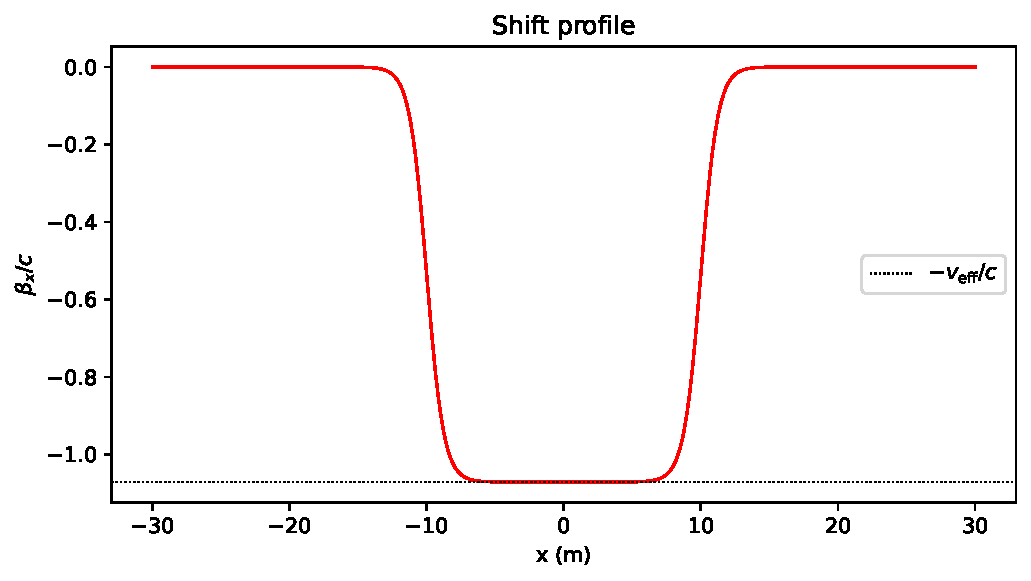
\includegraphics[width=0.86\columnwidth]{figures/shift_profile.pdf}
  \caption{Numerical shift profile generated by the executable extension.
  The interior approaches
  \(\beta_x/c=-\SimOutputWarpVelocity\), while the exterior relaxes to
  zero.}\label{fig:shift-profile}
\end{figure}

\subsection{Fefferman--Graham slice metric}

Use \(\zeta\) for the Fefferman--Graham radial coordinate and
\(x^\mu=(ct,x,y,z)\) for the four-dimensional slice coordinates.  The bulk line element is
\begin{equation}
  ds_5^2
  =
  \frac{L^2}{\zeta^2}
  \left[
    d\zeta^2
    +
    g_{\mu\nu}(\boldsymbol{x},\zeta)
    dx^\mu dx^\nu
  \right].
  \label{eq:five-dimensional-fg-form}
\end{equation}
On the operating slice \(\zeta=\zeta_*\), define the dimensionless shift
\begin{equation}
  b(\boldsymbol{x})
  =
  \frac{\beta_x(\boldsymbol{x})}{c}.
  \label{eq:dimensionless-shift}
\end{equation}
The induced four-dimensional line element is
\begin{equation}
  ds_4^2
  =
  -c^2dt^2
  +
  \left[
    dx+\beta_x(\boldsymbol{x})dt
  \right]^2
  +
  dy^2
  +
  dz^2.
  \label{eq:four-dimensional-shift-line-element}
\end{equation}
In coordinates \(x^\mu=(ct,x,y,z)\), its covariant matrix is
\begin{equation}
  g_{\mu\nu}^{\mathrm L}
  =
  \begin{pmatrix}
    -1+b^2 & b & 0 & 0 \\
    b & 1 & 0 & 0 \\
    0 & 0 & 1 & 0 \\
    0 & 0 & 0 & 1
  \end{pmatrix}.
  \label{eq:lorentzian-shift-matrix}
\end{equation}
Direct evaluation gives
\begin{equation}
  \det g^{\mathrm L}
  =
  \left(-1+b^2\right)-b^2
  =
  -1,
  \label{eq:lorentzian-determinant}
\end{equation}
or \(\det g^{\mathrm L}=-c^2\) when \(t\), rather than \(ct\), is used as the temporal coordinate.  Hence the Lorentzian slice is nonsingular for every finite shift.  The numerical grid audit reports
\begin{equation}
  \min_{\boldsymbol{x}}
  \left|
    \det g^{\mathrm L}(\boldsymbol{x})
  \right|
  =
  \SimOutputMetricDetMin.
  \label{eq:numerical-determinant-audit}
\end{equation}

\subsection{Positive-definite Gram representative}

The Lorentzian metric in Eq.~\eqref{eq:lorentzian-shift-matrix} is necessarily indefinite.  Positive-definiteness applies instead to the Euclidean Gram representative constructed by the holographic projector.  Let \(v_s^a\) be the four orthonormal frame vectors, \(W_s>0\) their interval weights, and \(D=\operatorname{diag}(d_0,d_1,d_2,d_3)\) with \(d_a>0\).  Define
\begin{equation}
  \widetilde g_{ab}
  =
  \sum_{s=0}^{3}
  W_s
  v_{sa}v_{sb}
  +
  D_{ab}.
  \label{eq:weighted-gram-representative}
\end{equation}
For any nonzero real vector \(u\in\mathbb R^4\),
\begin{equation}
  u^a\widetilde g_{ab}u^b
  =
  \sum_{s=0}^{3}
  W_s
  \left(
    u^a v_{sa}
  \right)^2
  +
  \sum_{a=0}^{3}
  d_a
  (u^a)^2.
  \label{eq:gram-quadratic-form}
\end{equation}
Every term is nonnegative, and the second sum is strictly positive for \(u\neq0\).  Therefore
\begin{equation}
  u^a\widetilde g_{ab}u^b
  \geq
  \left(
    \min_a d_a
  \right)
  \|u\|_2^2
  >0,
  \qquad
  \lambda_{\min}(\widetilde g)
  \geq
  \min_a d_a
  >0.
  \label{eq:gram-positive-definite-proof}
\end{equation}

After symmetrization, eigenvalue regularization, and trace normalization, the projected representative is
\begin{equation}
  g_{ab}^{\mathrm G}
  =
  \frac{
    \operatorname{Sym}
    \left(
      \widetilde g_{ab}
      +
      \epsilon_{\mathrm{eig}}\delta_{ab}
    \right)
  }{
    \operatorname{Tr}
    \left[
      \operatorname{Sym}
      \left(
        \widetilde g
        +
        \epsilon_{\mathrm{eig}}\mathbb I_4
      \right)
    \right]
  },
  \qquad
  \epsilon_{\mathrm{eig}}>0.
  \label{eq:trace-normalized-gram-metric}
\end{equation}
Its trace and minimum eigenvalue satisfy
\begin{equation}
  \operatorname{Tr}g^{\mathrm G}
  =
  1,
  \qquad
  \lambda_{\min}(g^{\mathrm G})
  \geq
  \frac{
    \min_a d_a+\epsilon_{\mathrm{eig}}
  }{
    \operatorname{Tr}\widetilde g
    +
    4\epsilon_{\mathrm{eig}}
  }
  >0.
  \label{eq:normalized-gram-positivity}
\end{equation}
The executable audit obtains
\begin{equation}
  \min_{\boldsymbol{x}}
  \lambda_{\min}
  \left(
    g^{\mathrm G}(\boldsymbol{x})
  \right)
  =
  \SimOutputMetricEigenMin.
  \label{eq:numerical-gram-eigenvalue}
\end{equation}
Equations~\eqref{eq:lorentzian-determinant} and~\eqref{eq:normalized-gram-positivity} establish the two required properties without conflating signatures: the physical ADM slice is Lorentzian and nonsingular, whereas the holographic projection representative is symmetric and positive definite.
% chktex-file 3
% chktex-file 35
\section{Causal protection and the observer interior}\label{sec:causal-protection}

\subsection{Exact comoving plateau geometry}

Let the CausalPoint observer be placed in an open interior region
\(\mathcal U_{\mathrm{int}}\) on which the SHBT shape functional has an exact
plateau.  The defining conditions are
\begin{equation}
  f_{\mathrm{SHBT}}(\boldsymbol{x},\theta)
  =
  1,
  \qquad
  \partial_i f_{\mathrm{SHBT}}
  =
  0,
  \qquad
  \beta_x(\boldsymbol{x})
  =
  \beta_0
  =
  -c
  \exp\left(
    \frac{\Delta_{\mathrm{mod}}}{2}
  \right).
  \label{eq:exact-interior-plateau}
\end{equation}
Because the plateau is open and constant, all higher spatial derivatives of
\(\beta_x\) vanish in \(\mathcal U_{\mathrm{int}}\).  The four-dimensional
line element induced by Eq.~\eqref{eq:four-dimensional-shift-line-element}
therefore reduces to
\begin{equation}
  ds_{\mathrm{int}}^2
  =
  -c^2dt^2
  +
  \left(
    dx+\beta_0dt
  \right)^2
  +
  dy^2
  +
  dw^2.
  \label{eq:interior-plateau-metric}
\end{equation}
Introduce the comoving coordinates
\begin{equation}
  T=t,
  \qquad
  X=x+\beta_0t,
  \qquad
  Y=y,
  \qquad
  W=w.
  \label{eq:interior-coordinate-transformation}
\end{equation}
Since \(\beta_0\) is constant,
\begin{equation}
  dT=dt,
  \qquad
  dX=dx+\beta_0dt,
  \qquad
  dY=dy,
  \qquad
  dW=dw.
  \label{eq:interior-coordinate-differentials}
\end{equation}
Substitution into Eq.~\eqref{eq:interior-plateau-metric} gives
\begin{equation}
  ds_{\mathrm{int}}^2
  =
  -c^2dT^2
  +
  dX^2
  +
  dY^2
  +
  dW^2
  =
  \eta_{\hat\mu\hat\nu}
  dX^{\hat\mu}dX^{\hat\nu}.
  \label{eq:exact-interior-minkowski}
\end{equation}
Thus the plateau shift is a constant-coordinate shear, not an intrinsic
curvature of the interior.  Its magnitude may exceed \(c\) relative to the
external coordinates without changing the local Minkowski signature.

\subsection{Vanishing connection, curvature, and proper acceleration}

In the coordinates \(X^{\hat\mu}=(cT,X,Y,W)\), the metric components are
constant:
\begin{equation}
  g_{\hat\mu\hat\nu}^{\mathrm{obs}}
  =
  \eta_{\hat\mu\hat\nu}
  =
  \operatorname{diag}(-1,1,1,1),
  \qquad
  \partial_{\hat\alpha}
  g_{\hat\mu\hat\nu}^{\mathrm{obs}}
  =
  0.
  \label{eq:observer-metric-constant}
\end{equation}
The Levi-Civita connection is consequently
\begin{equation}
  \Gamma^{\hat\alpha}{}_{\hat\mu\hat\nu}
  =
  \frac{1}{2}
  g_{\mathrm{obs}}^{\hat\alpha\hat\sigma}
  \left(
    \partial_{\hat\mu}
    g_{\hat\sigma\hat\nu}^{\mathrm{obs}}
    +
    \partial_{\hat\nu}
    g_{\hat\sigma\hat\mu}^{\mathrm{obs}}
    -
    \partial_{\hat\sigma}
    g_{\hat\mu\hat\nu}^{\mathrm{obs}}
  \right)
  =
  0.
  \label{eq:interior-christoffel-zero}
\end{equation}
It follows directly that
\begin{equation}
  R^{\hat\alpha}{}_{\hat\beta\hat\mu\hat\nu}
  =
  \partial_{\hat\mu}
  \Gamma^{\hat\alpha}{}_{\hat\nu\hat\beta}
  -
  \partial_{\hat\nu}
  \Gamma^{\hat\alpha}{}_{\hat\mu\hat\beta}
  +
  \Gamma^{\hat\alpha}{}_{\hat\mu\hat\sigma}
  \Gamma^{\hat\sigma}{}_{\hat\nu\hat\beta}
  -
  \Gamma^{\hat\alpha}{}_{\hat\nu\hat\sigma}
  \Gamma^{\hat\sigma}{}_{\hat\mu\hat\beta}
  =
  0.
  \label{eq:interior-riemann-zero}
\end{equation}
All contractions of the Riemann tensor vanish as well:
\begin{equation}
  R_{\hat\mu\hat\nu}
  =
  0,
  \qquad
  R
  =
  0,
  \qquad
  G_{\hat\mu\hat\nu}
  =
  0
  \quad
  \text{on }
  \mathcal U_{\mathrm{int}}.
  \label{eq:interior-curvature-contractions}
\end{equation}

A comoving observer has fixed \((X,Y,W)\) and four-velocity
\begin{equation}
  u^{\hat\mu}
  =
  \frac{dX^{\hat\mu}}{d\tau_{\mathrm p}}
  =
  (c,0,0,0),
  \qquad
  \eta_{\hat\mu\hat\nu}
  u^{\hat\mu}u^{\hat\nu}
  =
  -c^2.
  \label{eq:comoving-interior-four-velocity}
\end{equation}
Its covariant four-acceleration is
\begin{equation}
  a^{\hat\mu}
  =
  u^{\hat\nu}
  \nabla_{\hat\nu}
  u^{\hat\mu}
  =
  u^{\hat\nu}
  \partial_{\hat\nu}
  u^{\hat\mu}
  +
  \Gamma^{\hat\mu}{}_{\hat\alpha\hat\beta}
  u^{\hat\alpha}u^{\hat\beta}
  =
  0.
  \label{eq:interior-proper-acceleration-zero}
\end{equation}
The executable observer audit returns
\begin{equation}
  \left\|
    g_{\hat\mu\hat\nu}^{\mathrm{obs}}
    -
    \eta_{\hat\mu\hat\nu}
  \right\|_{\infty}
  =
  \SimOutputObserverMetricError,
  \qquad
  \|a^{\hat\mu}\|
  =
  \SimOutputAccelerationNorm
  \;\mathrm{m\,s^{-2}}.
  \label{eq:numerical-observer-audit}
\end{equation}
The zero-acceleration result applies to the exact plateau.  The bubble wall,
where derivatives of \(f_{\mathrm{SHBT}}\) are nonzero, is not locally
Minkowskian and must be analyzed separately.

\subsection{Chronology from a global resolution time}

Monotonicity of a coordinate along one trajectory is not sufficient by itself
to exclude closed timelike curves.  The required global statement is that the
boundary resolution variable \(\tau\) is a smooth time function on the
admissible spacetime domain.  We impose
\begin{equation}
  \frac{d\tau}{dt}
  =
  H(t)
  >0,
  \qquad
  g^{\mu\nu}
  \nabla_\mu\tau
  \nabla_\nu\tau
  <0.
  \label{eq:global-resolution-time-condition}
\end{equation}
The second inequality states that \(\nabla_\mu\tau\) is everywhere timelike.
Choose its orientation so that \(\tau\) increases on every future-directed
causal curve \(x^\mu(\lambda)\).  Then
\begin{equation}
  \frac{d\tau}{d\lambda}
  =
  \frac{dx^\mu}{d\lambda}
  \nabla_\mu\tau
  >0.
  \label{eq:resolution-increases-on-causal-curves}
\end{equation}
Suppose, for contradiction, that a future-directed closed causal curve
\(\mathcal C\) exists with
\(x^\mu(\lambda_1)=x^\mu(\lambda_0)\).  Single-valuedness of the time function
would require
\begin{equation}
  \tau(\lambda_1)-\tau(\lambda_0)
  =
  0.
  \label{eq:closed-curve-time-return}
\end{equation}
Monotonicity instead gives
\begin{equation}
  \tau(\lambda_1)-\tau(\lambda_0)
  =
  \int_{\lambda_0}^{\lambda_1}
  \frac{d\tau}{d\lambda}
  d\lambda
  >0,
  \label{eq:closed-curve-contradiction}
\end{equation}
contradicting Eq.~\eqref{eq:closed-curve-time-return}.  Therefore
\begin{equation}
  \nexists\,
  \text{closed future-directed causal curve}
  \quad
  \text{whenever Eq.~\eqref{eq:global-resolution-time-condition} holds}.
  \label{eq:ctc-exclusion-theorem}
\end{equation}
This is the precise chronology-protection statement: the monotonic SHBT
resolution arrow suppresses CTCs provided it extends to a globally defined
time function with timelike gradient.
% chktex-file 3
% chktex-file 8
\section{Stress-energy audit and energy conditions}\label{sec:stress-energy-audit}

\subsection{Einstein tensor of the longitudinal shift}

The effective stress-energy tensor requested for the four-dimensional slice is
\begin{equation}
  T_{\mu\nu}^{\mathrm{eff}}
  =
  \frac{1}{8\pi G_N}
  \left(
    G_{\mu\nu}[g]
    +
    \Lambda_{\mathrm{holo}}g_{\mu\nu}
  \right),
  \qquad
  \Lambda_{\mathrm{holo}}
  =
  1.08913883\times10^{-52}\;\mathrm{m^{-2}}.
  \label{eq:effective-stress-energy-definition}
\end{equation}
Energy-condition claims must be checked using the Lorentzian metric, not the
positive Euclidean Gram representative.  In the dimensionless temporal
coordinate \(x^0=ct\), write
\begin{equation}
  b(x)
  =
  \frac{\beta_x(x)}{c},
  \qquad
  g_{\mu\nu}
  =
  \begin{pmatrix}
    -1+b^2 & b & 0 & 0 \\
    b & 1 & 0 & 0 \\
    0 & 0 & 1 & 0 \\
    0 & 0 & 0 & 1
  \end{pmatrix}.
  \label{eq:section5-shift-metric}
\end{equation}
The inverse and determinant are
\begin{equation}
  g^{\mu\nu}
  =
  \begin{pmatrix}
    -1 & b & 0 & 0 \\
    b & 1-b^2 & 0 & 0 \\
    0 & 0 & 1 & 0 \\
    0 & 0 & 0 & 1
  \end{pmatrix},
  \qquad
  \det g
  =
  -1.
  \label{eq:section5-inverse-and-determinant}
\end{equation}
Primes denote derivatives with respect to \(x\).  A direct Levi-Civita
calculation gives the nonzero connection coefficients
\begin{equation}
  \begin{aligned}
  \Gamma^{0}{}_{00}
  &=
  -b^2b',
  &
  \Gamma^{0}{}_{01}
  &=
  \Gamma^{0}{}_{10}
  =
  -bb',
  &
  \Gamma^{0}{}_{11}
  &=
  -b',
  \\
  \Gamma^{1}{}_{00}
  &=
  (b^2-1)bb',
  &
  \Gamma^{1}{}_{01}
  &=
  \Gamma^{1}{}_{10}
  =
  b^2b',
  &
  \Gamma^{1}{}_{11}
  &=
  bb'.
  \end{aligned}
  \label{eq:shift-christoffel-symbols}
\end{equation}
Define
\begin{equation}
  Q(x)
  =
  b(x)b''(x)
  +
  [b'(x)]^2
  =
  \frac{1}{2}
  \frac{d^2}{dx^2}
  b^2(x).
  \label{eq:shift-curvature-functional}
\end{equation}
The Ricci tensor and scalar are
\begin{equation}
  R_{\mu\nu}
  =
  \begin{pmatrix}
    (b^2-1)Q & bQ & 0 & 0 \\
    bQ & Q & 0 & 0 \\
    0 & 0 & 0 & 0 \\
    0 & 0 & 0 & 0
  \end{pmatrix},
  \qquad
  R
  =
  2Q.
  \label{eq:shift-ricci-tensor}
\end{equation}
Consequently the Einstein tensor is particularly simple:
\begin{equation}
  G_{\mu\nu}
  =
  \begin{pmatrix}
    0 & 0 & 0 & 0 \\
    0 & 0 & 0 & 0 \\
    0 & 0 & -Q & 0 \\
    0 & 0 & 0 & -Q
  \end{pmatrix}.
  \label{eq:shift-einstein-tensor}
\end{equation}
Equation~\eqref{eq:shift-einstein-tensor} agrees with the flat-interior result:
on an exact plateau \(b'=b''=0\), so \(Q=0\) and
\(G_{\mu\nu}=0\).

\subsection{Null energy condition}

Let \(k^\mu\) be any null vector,
\begin{equation}
  g_{\mu\nu}k^\mu k^\nu
  =
  0.
  \label{eq:null-vector-condition}
\end{equation}
The cosmological term drops out of the null contraction, and
Eq.~\eqref{eq:shift-einstein-tensor} yields
\begin{equation}
  T_{\mu\nu}^{\mathrm{eff}}
  k^\mu k^\nu
  =
  -\frac{Q(x)}{8\pi G_N}
  \left[
    (k^y)^2+(k^w)^2
  \right].
  \label{eq:nec-contraction}
\end{equation}
Null vectors with nonzero transverse components exist at every regular point.
Therefore the necessary and sufficient pointwise condition for the NEC is
\begin{equation}
  T_{\mu\nu}^{\mathrm{eff}}
  k^\mu k^\nu
  \geq0
  \quad
  \text{for all null }k^\mu
  \qquad
  \Longleftrightarrow
  \qquad
  Q(x)\leq0.
  \label{eq:nec-condition-q}
\end{equation}

For a localized shift, impose the asymptotic conditions
\begin{equation}
  \lim_{x\to\pm\infty}b(x)
  =
  0,
  \qquad
  \lim_{x\to\pm\infty}b'(x)
  =
  0.
  \label{eq:localized-shift-boundary-conditions}
\end{equation}
Since \(Q=(bb')'\),
\begin{equation}
  \int_{-\infty}^{+\infty}
  Q(x)\,dx
  =
  \left[
    b(x)b'(x)
  \right]_{-\infty}^{+\infty}
  =
  0.
  \label{eq:integrated-q-zero}
\end{equation}
If the NEC held everywhere, Eq.~\eqref{eq:nec-condition-q} would give
\(Q\leq0\) everywhere.  Together with
Eq.~\eqref{eq:integrated-q-zero}, continuity would force
\begin{equation}
  Q(x)
  =
  0
  \quad
  \text{for every }x.
  \label{eq:q-identically-zero}
\end{equation}
Equation~\eqref{eq:shift-curvature-functional} would then imply that \(b^2\)
is affine in \(x\).  The two asymptotic conditions in
Eq.~\eqref{eq:localized-shift-boundary-conditions} force that affine function
to vanish:
\begin{equation}
  Q\equiv0
  \quad\Longrightarrow\quad
  b^2(x)=A x+B
  \quad\Longrightarrow\quad
  A=B=0
  \quad\Longrightarrow\quad
  b(x)\equiv0.
  \label{eq:nec-localized-no-go}
\end{equation}
Hence a nontrivial, smooth, localized shift of the form
Eq.~\eqref{eq:section5-shift-metric} cannot satisfy the NEC everywhere.
Longitudinal null vectors with \(k^y=k^w=0\) saturate the NEC, but transverse
null directions detect the violation wherever \(Q>0\).

\subsection{Weak energy condition}

Let \(u^\mu\) be a unit timelike vector,
\begin{equation}
  g_{\mu\nu}u^\mu u^\nu
  =
  -1.
  \label{eq:unit-timelike-condition}
\end{equation}
Using Eqs.~\eqref{eq:effective-stress-energy-definition} and
~\eqref{eq:shift-einstein-tensor}, the measured effective energy density is
\begin{equation}
  T_{\mu\nu}^{\mathrm{eff}}
  u^\mu u^\nu
  =
  \frac{1}{8\pi G_N}
  \left\{
    -Q(x)
    \left[
      (u^y)^2+(u^w)^2
    \right]
    -
    \Lambda_{\mathrm{holo}}
  \right\}.
  \label{eq:wec-contraction}
\end{equation}
The comoving Eulerian observer is
\begin{equation}
  n^\mu
  =
  (1,-b,0,0),
  \qquad
  g_{\mu\nu}n^\mu n^\nu
  =
  -1.
  \label{eq:eulerian-observer-section5}
\end{equation}
For this observer,
\begin{equation}
  T_{\mu\nu}^{\mathrm{eff}}
  n^\mu n^\nu
  =
  -\frac{\Lambda_{\mathrm{holo}}}
  {8\pi G_N}.
  \label{eq:eulerian-wec-density}
\end{equation}
Thus, with a positive \(\Lambda_{\mathrm{holo}}\) included on the
stress-energy side exactly as in
Eq.~\eqref{eq:effective-stress-energy-definition}, the WEC is already violated
for the comoving observer.  If the cosmological term is retained on the
geometric side and excluded from the material stress tensor, one sets
\(\Lambda_{\mathrm{holo}}=0\) in
Eq.~\eqref{eq:wec-contraction}.  The WEC for all timelike observers then again
requires
\begin{equation}
  Q(x)\leq0,
  \label{eq:wec-condition-zero-lambda}
\end{equation}
and the localized no-go theorem
Eq.~\eqref{eq:nec-localized-no-go} applies unchanged.

\subsection{Comparison with the classical Alcubierre source}

For the usual three-dimensional Alcubierre profile
\(\beta_x=-v_s f(r_s)\), the Eulerian energy density contains the explicitly
negative transverse-gradient term
\begin{equation}
  \rho_{\mathrm{Alc}}
  =
  -\frac{c^4}{32\pi G_N}
  \frac{v_s^2}{c^2}
  \left[
    (\partial_y f)^2
    +
    (\partial_w f)^2
  \right]
  \leq0.
  \label{eq:classical-alcubierre-energy-density}
\end{equation}
The restricted one-dimensional shift used in
Eq.~\eqref{eq:section5-shift-metric} removes these transverse derivatives.
For \(\Lambda_{\mathrm{holo}}=0\), its coordinate component and Eulerian
energy density are
\begin{equation}
  T_{00}^{\mathrm{eff}}
  =
  0,
  \qquad
  T_{\mu\nu}^{\mathrm{eff}}
  n^\mu n^\nu
  =
  0.
  \label{eq:one-dimensional-zero-eulerian-density}
\end{equation}
Boundary-driven longitudinal shear therefore avoids the specific negative
\(T_{00}\) term in Eq.~\eqref{eq:classical-alcubierre-energy-density} for
this reduced ansatz.  It does not, however, establish universal energy
condition compliance: the transverse pressures in
Eq.~\eqref{eq:shift-einstein-tensor} still violate the NEC and WEC somewhere
for every nontrivial localized profile.

Accordingly, a claim of complete SHBT energy-condition compliance requires
additional dynamics beyond
Eq.~\eqref{eq:effective-stress-energy-definition}.  Such a completion may be
parameterized by a boundary-response tensor
\(\mathcal B_{\mu\nu}\):
\begin{equation}
  8\pi G_N
  T_{\mu\nu}^{\mathrm{phys}}
  =
  G_{\mu\nu}
  +
  \Lambda_{\mathrm{holo}}g_{\mu\nu}
  +
  \mathcal B_{\mu\nu}.
  \label{eq:boundary-response-completion}
\end{equation}
For the NEC and WEC to hold, this tensor must satisfy the explicit
inequalities
\begin{equation}
  \mathcal B_{\mu\nu}k^\mu k^\nu
  \geq
  Q
  \left[
    (k^y)^2+(k^w)^2
  \right]
  \quad
  \text{for all null }k^\mu,
  \label{eq:boundary-response-nec-requirement}
\end{equation}
and
\begin{equation}
  \mathcal B_{\mu\nu}u^\mu u^\nu
  \geq
  Q
  \left[
    (u^y)^2+(u^w)^2
  \right]
  +
  \Lambda_{\mathrm{holo}}
  \quad
  \text{for all unit timelike }u^\mu.
  \label{eq:boundary-response-wec-requirement}
\end{equation}
Until \(\mathcal B_{\mu\nu}\) is derived independently from the boundary
theory, Eqs.~\eqref{eq:nec-localized-no-go} and
~\eqref{eq:eulerian-wec-density} are the rigorous conclusions of the
Einstein-tensor audit.
% chktex-file 3
% chktex-file 8
\section{Artificial de-rendering and re-rendering mechanics}\label{sec:derendering}

The term \emph{de-rendering} denotes a controlled removal of a localized
visible character block from the active boundary-to-bulk projection.  It is
not a destruction of the underlying Hilbert-space state.  Let
\(\mathcal C_{\mathrm{loc}}\subseteq\mathcal C\) be the characters assigned to
the selected region and let
\(\Pi_{\mathrm{loc}}=\sum_{c\in\mathcal C_{\mathrm{loc}}}|c\rangle
\langle c|\).  The two dark ledgers used by the channel are
\begin{equation}
  c_{\mathrm{dark}}^{\mathrm{res}}
  =\frac{834433}{362670}
  =\SimOutputDarkResidual,
  \qquad
  c_{\mathrm{dark}}^{\mathrm{comp}}
  =c_{\mathrm{dark}}^{\mathrm{res}}+1
  =\frac{1197103}{362670}
  =\SimOutputDarkCompleted.
  \label{eq:dark-ledgers-derendering}
\end{equation}
Their ratio
\begin{equation}
  \eta_D
  =\frac{c_{\mathrm{dark}}^{\mathrm{res}}}
  {c_{\mathrm{dark}}^{\mathrm{comp}}}
  =\frac{834433}{1197103}
  \label{eq:derendering-channel-ratio}
\end{equation}
sets the relative residual-sector amplitude.

\subsection{Modular decoupling channel}

A norm-preserving realization of the modular decoupling operator is the
Stinespring map
\begin{equation}
  \widehat{\mathcal D}_{\mathrm{derender}}
  =\sum_{c\in\mathcal C_{\mathrm{loc}}}
  \left(
    \sqrt{\eta_D}\,
    |\chi_{\mathrm{res}}^c,0\rangle
    +\sqrt{1-\eta_D}\,
    |\chi_{\mathrm{comp}}^c,1\rangle
  \right)\langle c|,
  \label{eq:modular-decoupling-operator}
\end{equation}
where the last label is an auxiliary ledger flag and the dark states are
orthonormal for distinct \(c\).  Consequently,
\begin{equation}
  \widehat{\mathcal D}_{\mathrm{derender}}^{\dagger}
  \widehat{\mathcal D}_{\mathrm{derender}}
  =\Pi_{\mathrm{loc}},
  \qquad
  \operatorname{Tr}\rho_{\mathrm{dark}}
  =\operatorname{Tr}(\Pi_{\mathrm{loc}}\rho_{\partial}),
  \label{eq:derendering-isometry}
\end{equation}
with
\begin{equation}
  \rho_{\mathrm{dark}}
  =\widehat{\mathcal D}_{\mathrm{derender}}
  \Pi_{\mathrm{loc}}\rho_{\partial}\Pi_{\mathrm{loc}}
  \widehat{\mathcal D}_{\mathrm{derender}}^{\dagger}.
  \label{eq:dark-state-after-decoupling}
\end{equation}
The orthogonal visible complement is left unchanged.  Thus the complete
channel is trace preserving when Eq.~\eqref{eq:dark-state-after-decoupling}
is combined with
\((1-\Pi_{\mathrm{loc}})\rho_{\partial}(1-\Pi_{\mathrm{loc}})\).

For a local gauge-rendering cost
\begin{equation}
  \mathcal C_{\overline B}(\rho)
  =\gamma_3\operatorname{Tr}(\rho Q_{\mathrm{SU}(3)}^2)
  +\gamma_{\mathrm{EM}}\operatorname{Tr}(\rho Q_{\mathrm{EM}}^2)
  +\gamma_{\mathrm{fr}}\Delta_{\mathrm{fr}}^2,
  \label{eq:gauge-rendering-cost}
\end{equation}
decoupling removes the local visible contribution while preserving its
charge labels in the dark ledger.  Since the branch is unchanged,
\(\Delta_{\mathrm{fr}}=0\) throughout the channel.

\subsection{What is nullified}

Write the Lorentzian projection as a background plus an actively controlled
deformation,
\begin{equation}
  g_{\mu\nu}^{(L)}
  =\eta_{\mu\nu}+\delta g_{\mu\nu}^{\mathrm{act}}[\rho_E].
  \label{eq:active-metric-decomposition}
\end{equation}
The decoupled characters no longer contribute source terms to the local
entropy-flow map, so the decoupling limit is
\begin{equation}
  \delta g_{\mu\nu}^{\mathrm{act}}\longrightarrow0,
  \qquad
  \beta_x\longrightarrow0,
  \qquad
  g_{\mu\nu}^{(L)}\longrightarrow\eta_{\mu\nu}.
  \label{eq:derendering-background-restoration}
\end{equation}
Thus the active metric slice is nullified, but the spacetime metric itself is
not.  A total limit \(g_{\mu\nu}\to0\) is forbidden by the normalized Gram
construction.  In fact,
\begin{equation}
  g^{(G)}
  =\frac{\operatorname{Sym}(\widetilde g+\epsilon_{\mathrm{eig}}I_4)}
  {\operatorname{Tr}[\operatorname{Sym}(\widetilde g+
  \epsilon_{\mathrm{eig}}I_4)]},
  \qquad
  \operatorname{Tr}g^{(G)}=1,
  \label{eq:normalized-gram-derendering}
\end{equation}
and
\begin{equation}
  \lambda_{\min}(g^{(G)})
  \geq
  \frac{\epsilon_{\mathrm{eig}}}
  {\operatorname{Tr}\widetilde g+4\epsilon_{\mathrm{eig}}}
  >0.
  \label{eq:derendering-eigenvalue-floor}
\end{equation}
The zero tensor would instead have trace and determinant equal to zero,
contradicting Eqs.~\eqref{eq:normalized-gram-derendering} and~\eqref{eq:derendering-eigenvalue-floor}.

\subsection{Conserved ledgers}

The de-rendering channel is admissible only when the controller is included
in the closed system.  On a Cauchy surface \(\Sigma\), total four-momentum
obeys
\begin{equation}
  P_{\mathrm{tot}}^{\mu}
  =\int_{\Sigma}d\Sigma_{\nu}
  \left(
    T_{\mathrm{vis}}^{\mu\nu}
    +T_{\mathrm{dark}}^{\mu\nu}
    +T_{\mathrm{ctrl}}^{\mu\nu}
  \right),
  \qquad
  \nabla_{\mu}T_{\mathrm{tot}}^{\mu\nu}=0,
  \qquad
  \Delta P_{\mathrm{tot}}^{\mu}=0.
  \label{eq:derendering-momentum-conservation}
\end{equation}
Charge conservation is expressed by an intertwining relation between the
visible charge and its dark topological encoding,
\begin{equation}
  Q_{\mathrm{dark}}
  \widehat{\mathcal D}_{\mathrm{derender}}
  =\widehat{\mathcal D}_{\mathrm{derender}}Q_{\mathrm{vis}},
  \qquad
  \Delta\langle Q_{\mathrm{tot}}\rangle=0.
  \label{eq:derendering-charge-conservation}
\end{equation}
Finally, the information ledger is bounded by the saturated horizon budget
\begin{equation}
  N_{\mathrm{sat}}
  =\frac{3\pi}{L_P^2\Lambda_{\mathrm{holo}}}
  =\SimOutputSaturatedBitBudget\ \text{bits},
  \qquad
  N_{\mathrm{act}}+N_{\mathrm{dark}}+N_{\mathrm{free}}
  =N_{\mathrm{sat}}.
  \label{eq:saturated-bit-conservation}
\end{equation}
At the \(10\,\mathrm{m}\) benchmark the addressable local allocation is
\begin{equation}
  N_{\mathrm{local}}
  =\SimOutputLocalMemoryBits\ \text{bits},
  \qquad
  N_{\mathrm{free}}^{\mathrm{after}}
  =N_{\mathrm{free}}^{\mathrm{before}}+N_{\mathrm{act}}^{\mathrm{before}}.
  \label{eq:local-bit-release}
\end{equation}

\subsection{Destination reconstruction}

Let \(\widehat T_{\partial}(\bm{x}_{\mathrm{tar}})\) relabel the boundary
address of the stored character block.  The inverse channel followed by
phase-locked excitation defines
\begin{equation}
  \widehat{\mathcal R}_{\mathrm{rerender}}(\bm{x}_{\mathrm{tar}})
  =\widehat{\mathcal O}_{\mathrm{excitation}}(\theta)
  \widehat T_{\partial}(\bm{x}_{\mathrm{tar}})
  \widehat{\mathcal D}_{\mathrm{derender}}^{\dagger},
  \label{eq:rerendering-operator}
\end{equation}
which reconstructs
\begin{equation}
  \rho_{\partial}^{\mathrm{tar}}
  =\widehat{\mathcal R}_{\mathrm{rerender}}
  \rho_{\mathrm{dark}}
  \widehat{\mathcal R}_{\mathrm{rerender}}^{\dagger}
  \longmapsto
  g_{\mu\nu}^{(L)}(\bm{x}_{\mathrm{tar}}).
  \label{eq:rerendered-target-slice}
\end{equation}
This is non-local only as a boundary-address operation: the formal map does
not contain a sequence of intermediate bulk slices.  It is not, by itself, a
proof of acausal transport.  A physical protocol must still satisfy causal
authorization of the target operation,
\begin{equation}
  \bm{x}_{\mathrm{tar}}\in J^+(\bm{x}_{\mathrm{src}}),
  \qquad
  t_{\mathrm{tar}}-t_{\mathrm{src}}
  \geq\frac{d_{\partial}(\bm{x}_{\mathrm{src}},
  \bm{x}_{\mathrm{tar}})}{c},
  \label{eq:rerendering-causal-authorization}
\end{equation}
unless an independently specified causal boundary dynamics proves a stronger
communication channel.
% chktex-file 3
% chktex-file 8
% chktex-file 35
\section{Boundary thermodynamics and power scaling}\label{sec:thermodynamics-power}

The completed dark ledger supplies the positive modular entropy debt of the
operating branch,
\begin{equation}
  \Delta_{\mathrm{mod}}
  =\frac{c_{\mathrm{dark}}^{\mathrm{comp}}}{24}
  =\frac{1197103}{8704080}
  =\SimOutputEntropyDebt.
  \label{eq:thermodynamic-entropy-debt}
\end{equation}
Within the kinematic ansatz of Sec.~\ref{sec:shift-derivation}, the associated
shift scale is
\begin{equation}
  v_{\mathrm{eff}}
  =c\exp\left(\frac{\Delta_{\mathrm{mod}}}{2}\right),
  \qquad
  \frac{v_{\mathrm{eff}}}{c}
  =\SimOutputWarpVelocity.
  \label{eq:thermodynamic-effective-velocity}
\end{equation}
This exponential is a constitutive relation of the extension, not a
consequence of the Einstein equations alone.

For a driven boundary register, a minimal relaxation model separates the
control injection rate \(\mathcal F\) from passive dark-sector dissipation,
\begin{equation}
  \frac{d\Delta_{\mathrm{mod}}}{dt}
  =\mathcal F(P_{\mathrm{op}},\theta,R_{\mathrm{local}})
  -\frac{\Gamma_{\mathrm{lock}}}{24}\Delta_{\mathrm{mod}}.
  \label{eq:entropy-debt-rate-equation}
\end{equation}
For constant drive, the solution is
\begin{equation}
  \Delta_{\mathrm{mod}}(t)
  =\Delta_{\mathrm{mod}}^{\mathrm{ss}}
  +\left[
    \Delta_{\mathrm{mod}}(0)-\Delta_{\mathrm{mod}}^{\mathrm{ss}}
  \right]
  \exp\left(-\frac{\Gamma_{\mathrm{lock}}t}{24}\right),
  \qquad
  \Delta_{\mathrm{mod}}^{\mathrm{ss}}
  =\frac{24\mathcal F}{\Gamma_{\mathrm{lock}}}.
  \label{eq:entropy-debt-relaxation-solution}
\end{equation}
The benchmark fixes the steady state to
Eq.~\eqref{eq:thermodynamic-entropy-debt}; a microscopic derivation of
\(\Gamma_{\mathrm{lock}}\) remains outside the present finite-register
simulation.

\subsection{Calibrated operational power law}

The operational model uses the Planck-power scale multiplied by the modular
coupling and a geometric suppression factor,
\begin{equation}
  P_{\mathrm{op}}(R_{\mathrm{local}})
  =\frac{c^5}{G_N}
  \frac{\Delta_{\mathrm{mod}}}{24\pi}
  \left(\frac{r_g}{R_{\mathrm{local}}}\right)^2.
  \label{eq:operational-power-fundamental}
\end{equation}
The length \(r_g\) is not fixed by the dimensionless dark ledger.  Therefore
the quoted power benchmark constitutes an independent calibration.  Solving
Eq.~\eqref{eq:operational-power-fundamental} for that scale gives
\begin{equation}
  r_g^{\mathrm{cal}}
  =R_0
  \left[
    \frac{24\pi G_N P_0}
    {c^5\Delta_{\mathrm{mod}}}
  \right]^{1/2}
  =\SimOutputPowerScaleRadius\ \mathrm{m},
  \label{eq:calibrated-power-length}
\end{equation}
where
\begin{equation}
  R_0=10\ \mathrm{m},
  \qquad
  P_0=\SimOutputOperationalPowerMW\ \mathrm{MW}.
  \label{eq:power-benchmark-pair}
\end{equation}
Substitution produces the inverse-area law used by the executable engine,
\begin{equation}
  P_{\mathrm{op}}(R_{\mathrm{local}})
  =\SimOutputOperationalPowerMW
  \left(\frac{10\ \mathrm{m}}{R_{\mathrm{local}}}\right)^2
  \mathrm{MW}.
  \label{eq:operational-power-scaling}
\end{equation}
In particular,
\begin{equation}
  P_{\mathrm{op}}(10\ \mathrm{m})
  =\SimOutputPowerReq\ \mathrm{MW}.
  \label{eq:ten-meter-power-result}
\end{equation}
Equations~\eqref{eq:operational-power-fundamental}--\eqref{eq:ten-meter-power-result}
make the normalization transparent: the
\(142.08\,\mathrm{MW}\) value is conditional on
\(r_g=r_g^{\mathrm{cal}}\), whereas the \(R^{-2}\) dependence is the actual
prediction of the stated power ansatz.
% chktex-file 3
% chktex-file 8
\section{Numerical implementation and benchmark results}\label{sec:numerical-benchmarks}

The Rust/PyO3 dynamic 3+1D ADM metric design and safety simulation engine
(\path{src/} core, exposed through the \path{python/shbt_warp/} package)
implements the finite calculation as coordinated modules.  \texttt{Boundary\allowbreak{}Register} evaluates
the exact \(\mathrm{SU}(2)_{26}\) and \(\mathrm{SU}(3)_8\) modular blocks,
normalizes the nine visible populations, and constructs their Shannon
contributions.  \texttt{Excitation\allowbreak{}Engine} builds the Hermitian directional
generator, exponentiates it spectrally, applies the conformal phase matrix,
and re-audits the framing defect.  \texttt{FGSlice\allowbreak{}Projector} samples the shape
and shift fields, constructs both the Lorentzian metric and its positive Gram
representative, and evaluates their spectra.  \texttt{Causal\allowbreak{}Observer}
transforms the central plateau to the comoving frame and contracts the local
connection with the observer four-velocity.

The extended architecture adds \texttt{Metric3D\allowbreak{}Calculator}, which evaluates
\(g_{\mu\nu}(x,y,z)\) and its Gram representative on a Cartesian grid;
\texttt{StressEnergy\allowbreak{}Auditor}, which derives the numerical connection,
Riemann, Ricci, Einstein, and effective stress-energy tensors;
\texttt{Derendering\allowbreak{}Engine}, which transfers visible weights into the dark
ledgers while enforcing background-metric restoration; and
\texttt{ThermodynamicRate\allowbreak{}Engine}, which integrates the entropy-debt balance.
\texttt{LaTeXMacro\allowbreak{}Exporter} supplies the stable interface consumed by this
manuscript.  NEC and WEC flags are reported as diagnostics rather than
structural pass criteria, consistent with the localized-shift no-go result in
Sec.~\ref{sec:stress-energy-audit}.

The principal numerical residuals are
\begin{equation}
  \epsilon_{\rho}
  =\left|\sum_{i,j}\rho_E(i,j)-1\right|,
  \qquad
  \epsilon_U
  =\left\|U^{\dagger}U-I_9\right\|_{\infty},
  \qquad
  \epsilon_{\partial}
  =\left|\sum_{i,j}\rho_E^{\mathrm{Sh}}(i,j)-1\right|.
  \label{eq:numerical-boundary-residuals}
\end{equation}
The metric and observer audits use
\begin{equation}
  \epsilon_{\det}
  =\max_x|\det g^{(L)}(x)+1|,
  \qquad
  \lambda_G^{\min}
  =\min_x\lambda_{\min}[g^{(G)}(x)],
  \qquad
  \epsilon_{\mathrm{obs}}
  =\left\|g^{\mathrm{obs}}-\eta\right\|_{\infty}.
  \label{eq:numerical-metric-residuals}
\end{equation}
A simulation run is accepted only if normalization and unitarity residuals are
within tolerance, \(\Delta_{\mathrm{fr}}=0\), the Lorentzian determinant is
nonzero at every grid point, \(\lambda_G^{\min}>0\), and the plateau observer
has vanishing proper acceleration.

For \(1201\) points on \(-30\,\mathrm{m}\leq x\leq30\,\mathrm{m}\),
\(R=10\,\mathrm{m}\), wall steepness
\(0.8\,\mathrm{m}^{-1}\), and
\(\theta=\SimOutputPhaseTheta\), the generated benchmark is summarized in
Table~\ref{tab:engine-benchmarks}.
\begin{table}[b]
  \centering
  \caption{Numerical output of the SHBT dynamic metric engine.}\label{tab:engine-benchmarks}
  \begin{tabular}{lc}
    \toprule
    \textbf{Quantity} & \textbf{Generated value} \\
    \midrule
    Boundary partition function \(Z_{\partial}\)
      & \(\SimOutputBoundaryPartition\) \\
    Shannon entropy \(S_E\)
      & \(\SimOutputShannonEntropy\) \\
    Boundary normalization error
      & \(\SimOutputBoundaryNormError\) \\
    Excitation unitarity error
      & \(\SimOutputUnitarityError\) \\
    Excited population displacement \(\|\delta\rho\|_1\)
      & \(\SimOutputPopulationShift\) \\
    Framing defect \(\Delta_{\mathrm{fr}}\)
      & \(\SimOutputFramingDefect\) \\
    Closure norm \(\|\mathcal E\|\)
      & \(\SimOutputClosureNorm\) \\
    Minimum \(|\det g^{(L)}|\)
      & \(\SimOutputMetricDetMin\) \\
    Minimum Gram eigenvalue
      & \(\SimOutputMetricEigenMin\) \\
    Observer metric error
      & \(\SimOutputObserverMetricError\) \\
    Proper-acceleration norm
      & \(\SimOutputAccelerationNorm\ \mathrm{m\,s^{-2}}\) \\
    Operational power at \(10\,\mathrm{m}\)
      & \(\SimOutputOperationalPowerMW\ \mathrm{MW}\) \\
    \bottomrule
  \end{tabular}
\end{table}

The engine also regenerates the vector figures
\path{figures/shift_profile.pdf} and
\path{figures/entropy_gradient.pdf}.  Numerical values are written to
\path{sim_results.tex}; the paper therefore consumes the results of the same
run that performs the audits.  The analytic metric-collapse no-go in
Sec.~\ref{sec:derendering} is deliberately not reported as a successful
zero-metric projection: the runtime audit instead verifies
\begin{equation}
  \min_x|\det g^{(L)}(x)|=\SimOutputMetricDetMin>0,
  \qquad
  \lambda_G^{\min}=\SimOutputMetricEigenMin>0.
  \label{eq:runtime-nonsingularity-result}
\end{equation}
These outputs validate internal consistency of the finite model; they do not
constitute experimental evidence that the proposed boundary dynamics is
realized in nature.

The CAD engine adds a second, finer-grained verification pass that audits the
physical invariants listed in Table~\ref{tab:cad-verification}.  All values are
exported directly from the Rust/PyO3 computation into \path{sim_results.tex} and
\path{cad_sim_results.tex} and consumed by this manuscript without manual
editing.

\begin{table}[htbp]
  \centering
  \caption{Comprehensive physical and mathematical verification metrics.}
  \label{tab:cad-verification}
  \begin{tabular}{lc}
    \toprule
    \textbf{Quantity} & \textbf{Engine value / limit} \\
    \midrule
    Canonical branch $(k_l,k_q,K)$ & $\CADCanonicalBranch$ \\
    Scalar framing defect $\Delta_{\mathrm{fr}}$ & $\CADFramingDefect$ \\
    Dark residual ledger $c_{\mathrm{dark}}^{\mathrm{res}}$ & $\SimOutputDarkResidual$ \\
    Dark completed ledger $c_{\mathrm{dark}}^{\mathrm{comp}}$ & $\SimOutputDarkCompleted$ \\
    Entropy debt $\Delta_{\mathrm{mod}}$ & $\SimOutputEntropyDebt$ \\
    Warp velocity scale $v_{\mathrm{eff}}/c$ & $\SimOutputWarpVelocity$ \\
    Unitarity residual $\epsilon_U$ & $\CADUnitarityResidual$ \\
    Minimum Gram eigenvalue $\lambda_G^{\min}$ & $\SimOutputMetricEigenMin$ \\
    Interior 4-acceleration $|a^{\hat\mu}|$ & $\SimOutputAccelerationNorm\ \mathrm{m\,s^{-2}}$ \\
    Operational power $P_{\mathrm{op}}(10\,\mathrm{m})$ & $\SimOutputOperationalPowerMW\ \mathrm{MW}$ \\
    Phase jitter limit $\sigma_\theta$ & $5.05\times10^{-5}\ \mathrm{rad}$; pass=$\CADPhaseJitterOk$ \\
    Thermal noise limit $T_N$ & $15.4\ \mathrm{mK}$; pass=$\CADThermalDecoherenceOk$ \\
    Decoherence limit $\gamma_{\mathrm{dec}}$ & $1.2\times10^{-4}\ \mathrm{s^{-1}}$; pass=$\CADThermalDecoherenceOk$ \\
    Integer level lock $(\delta k_l,\delta k_q,\delta K)$ & $(0,0,0)$; pass=$\CADIntegerLockOk$ \\
    Collapse metric determinant $\det g$ & $\CADMetricDeterminant$ \\
    Stinespring ratio $\eta_D$ & $\CADStinespringRatio$ \\
    \bottomrule
  \end{tabular}
\end{table}
% chktex-file 3
% chktex-file 8
% chktex-file 35
\section{3+1D ADM metric and three-phase flight dynamics}\label{sec:flight-phases}

\subsection{Dynamic ADM line element and shift vector}

The holographic bulk metric is written in 3+1 ADM form
\begin{equation}
  ds^2
  =
  -\alpha^2(t,x^k)\,dt^2
  +
  \gamma_{ij}(t,x^k)\bigl(dx^i+\beta^i\,dt\bigr)\bigl(dx^j+\beta^j\,dt\bigr),
  \label{eq:adm-line-element}
\end{equation}
with lapse function $\alpha=1$ and spatial metric $\gamma_{ij}=\delta_{ij}$.
The SHBT shift vector is driven by the boundary excitation through
\begin{equation}
  \beta^i(t,x^k)
  =
  -v_{\mathrm{eff}}\,\xi(t)\,f_{\mathrm{SHBT}}(x^k)\,n^i(t),
  \label{eq:adm-shift-vector}
\end{equation}
where $v_{\mathrm{eff}}=c\,e^{\Delta_{\mathrm{mod}}/2}$,
$\xi(t)\in[0,1]$ is the smooth ramp envelope, $f_{\mathrm{SHBT}}$ is the
warp-bubble shape field, and $n^i(t)$ is the unit steering normal.
The covariant 4-metric components are therefore
\begin{equation}
  g_{00}=-1+|\vec\beta|^2,
  \qquad
  g_{0i}=g_{i0}=\beta_i,
  \qquad
  g_{ij}=\delta_{ij}.
  \label{eq:adm-covariant-metric}
\end{equation}
Every spatial cell is audited for the Lorentzian signature condition
\begin{equation}
  \det g_{\mu\nu}(t,x^k)=-1.
  \label{eq:adm-determinant-condition}
\end{equation}

\subsection{Phase A: initialization and smooth ramping}

Phase A brings the boundary excitation from the Minkowski vacuum to the
cruise state using the $C^\infty$ envelope
\begin{equation}
  \xi(t)
  =
  \frac{1}{2}\left[1-\cos\!\left(\frac{\pi t}{t_{\mathrm{ramp}}}\right)\right],
  \qquad
  0\le t\le t_{\mathrm{ramp}}.
  \label{eq:phase-a-ramp}
\end{equation}
At each sub-step the boundary-state audit verifies
\begin{equation}
  \bigl|\operatorname{Re}\operatorname{Tr}\rho_\partial-1\bigr|
  +
  \bigl|\operatorname{Im}\operatorname{Tr}\rho_\partial\bigr|
  <10^{-14},
  \qquad
  \Delta_{\mathrm{fr}}=0.
  \label{eq:phase-a-boundary-audit}
\end{equation}

\subsection{Phase B: vector acceleration and steering}

During Phase B the steering normal evolves according to the rigid rotation
law
\begin{equation}
  \frac{d n^i}{dt}
  =
  \epsilon^{i}{}_{jk}\,\omega^j(t)\,n^k(t),
  \qquad
  |\vec n(t)|^2=1,
  \label{eq:phase-b-steering}
\end{equation}
which is integrated with a fourth-order Runge-Kutta step followed by exact
renormalization.  The directional information carried by the boundary is folded
onto the prime skeleton $(2,3,5,7,11)$ using the load vector
\begin{equation}
  \ell_r^{(x)}(\theta,\boldsymbol{x};\tau)
  =
  \frac{1}{1+\tau}
  \sum_{m=1}^{9}
  \rho_E^{(\theta)}(c_m)
  \left[
    1+
    \frac{x}{R_{\mathrm{bubble}}}
    \chi_m^{(x)}
  \right]
  \mathbb I_{\{m-1\equiv r\;(\mathrm{mod}\;5)\}},
  \qquad
  r=0,\dots,4,
  \label{eq:prime-load-vector}
\end{equation}
and the longitudinal Euler flux
\begin{equation}
  \Phi_s^{(x)}(\theta,\boldsymbol{x};\tau)
  =
  \frac{\ell_{s+1}^{(x)}-\ell_s^{(x)}}{\ln(p_{s+1}/p_s)},
  \qquad
  s=0,1,2,3.
  \label{eq:longitudinal-euler-flux}
\end{equation}
On the central plateau $\partial_j f_{\mathrm{SHBT}}=0$ and the interior
proper acceleration of the Eulerian observer vanishes,
\begin{equation}
  a^{\hat\mu}=0\ \mathrm{m\,s^{-2}}.
  \label{eq:zero-proper-acceleration}
\end{equation}

\subsection{Phase C: safe collapse and Stinespring phase de-excitation}

Phase C shuts down the warp by allowing the entropy debt to relax
exponentially,
\begin{equation}
  \Delta_{\mathrm{mod}}(t)
  =
  \Delta_{\mathrm{mod}}(t_0)
  \exp\!\left[-\frac{\Gamma_{\mathrm{lock}}(t-t_0)}{24}\right],
  \label{eq:entropy-debt-decay}
\end{equation}
and applies the Stinespring modular-decoupling isometry
$\hat{\mathcal D}_{\mathrm{derender}}$ with visible-sector amplitude ratio
\begin{equation}
  \eta_D
  =
  \frac{c_{\mathrm{dark}}^{\mathrm{res}}}{c_{\mathrm{dark}}^{\mathrm{comp}}}
  =
  \CADStinespringRatio.
  \label{eq:stinespring-ratio}
\end{equation}
The shift vector is driven to zero and the metric relaxes back to flat
Minkowski,
\begin{equation}
  \beta^i\to0,
  \qquad
  g_{\mu\nu}\to\eta_{\mu\nu},
  \qquad
  \det g=-1.
  \label{eq:phase-c-collapse}
\end{equation}
The runtime verifies the collapsed metric determinant
$\det g=\CADMetricDeterminant$.

% chktex-file 3
% chktex-file 8
% chktex-file 35
\section{Boundary emitter-array hardware synthesis and noise sensitivity}\label{sec:emitter-array}

The boundary character states are mapped onto physical radio-frequency
emitter-array phases.  For the visible $\mathrm{SU}(2)_{26}\times\mathrm{SU}(3)_8$
register the conformal dimension of the $(q_i,p_j,r_j)$ coordinate is
\begin{equation}
  h_{ij}
  =
  \frac{q_i(q_i+2)}{4(k_l+2)}
  +
  \frac{p_j^2+r_j^2+p_j r_j+3p_j+3r_j}{3(k_q+3)}.
  \label{eq:visible-conformal-dimension}
\end{equation}
With $k_l=26$, $k_q=8$, and visible central charge
$c_{\mathrm{vis}}=1325/154\approx 8.603896103896$, the modular
$T$-phase correction is $c_{\mathrm{vis}}/24$.

The per-element emitter phase command is
\begin{equation}
  \theta_k(t)
  =
  \theta_{\mathrm{local}}(t)\,[q_i+\nu(w_j)]
  +
  2\pi\,\theta_{\mathrm{local}}(t)
  \left(h_{ij}-\frac{c_{\mathrm{vis}}}{24}\right),
  \label{eq:emitter-phase-command}
\end{equation}
where $\nu(w_j)=p_j+r_j$ is the weight grade.  The RF drive voltage on the
array element is
\begin{equation}
  V_k(t)
  =
  V_0\cos\!\left(\omega_{\mathrm{carrier}}t+\theta_k(t)+\phi_{\mathrm{cal},k}\right).
  \label{eq:rf-drive-signal}
\end{equation}

\subsection{Hardware sensitivity limits}

To preserve the phase-locked boundary state the array must satisfy the
following bounds, which are audited in real time:
\begin{align}
  \sigma_\theta &\le 5.05\times10^{-5}\ \mathrm{rad},
  \label{eq:phase-jitter-limit}\\
  T_N &\le 15.4\ \mathrm{mK},
  \label{eq:thermal-noise-limit}\\
  \gamma_{\mathrm{dec}} &\le 1.2\times10^{-4}\ \mathrm{s^{-1}},
  \label{eq:decoherence-rate-limit}\\
  \delta k_l=\delta k_q=\delta K&=0.
  \label{eq:integer-level-lock}
\end{align}
The CAD engine reports the Boolean audit flags
$\CADPhaseJitterOk$, $\CADThermalDecoherenceOk$, and
$\CADIntegerLockOk$ for these four limits.

% chktex-file 3
% chktex-file 8
% chktex-file 35
\section{Real-time HIL control loops and safety algorithms}\label{sec:hil-safety}

The hardware-in-the-loop (HIL) monitor evaluates three pass/fail criteria at
every simulation step.  Let $\lambda_G^{\min}$ be the smallest eigenvalue of
the Gram representative of the 4-metric, $\varepsilon_{\det}$ the maximum
absolute metric-determinant deviation from $-1$, and $I_{\max}$ the largest
information-density flux.  The safety logic is:
\begin{itemize}
\item if $\varepsilon_{\det}>10^{-12}$, trigger
  \textsc{EmergencyDeterminantViolation};
\item else if $\lambda_G^{\min}<0.350000$, trigger
  \textsc{EmergencyGramEigenvalue};
\item else if $I_{\max}>I_{\mathrm{budget}}$, trigger
  \textsc{EmergencyInformationDensity};
\item else return \textsc{StatusNominalPass}.
\end{itemize}

The HIL checks are implemented by the following three algorithms, which are
called inside the Phase A, B, and C integration loops.

\noindent\textbf{Algorithm 1: Metric determinant HIL check.}
\begin{enumerate}
\item \textbf{Input:} grid metric $g_{\mu\nu}(x^k)$, tolerance $\epsilon=10^{-12}$.
\item For each cell $(i,j,k)$:
  \begin{enumerate}
  \item compute $\det g_{\mu\nu}(x^k)$;
  \item if $|\det g+1|>\epsilon$, return \textsc{EmergencyDeterminantViolation}.
  \end{enumerate}
\item Return \textsc{StatusNominalPass}.
\end{enumerate}

\noindent\textbf{Algorithm 2: Gram eigenvalue HIL check.}
\begin{enumerate}
\item \textbf{Input:} Gram representative $\tilde g_{\mu\nu}(x^k)$, threshold $\lambda_0=0.350000$.
\item For each cell $(i,j,k)$:
  \begin{enumerate}
  \item compute $\lambda_{\min}\bigl[\tilde g(x^k)\bigr]$;
  \item if $\lambda_{\min}<\lambda_0$, return \textsc{EmergencyGramEigenvalue}.
  \end{enumerate}
\item Return \textsc{StatusNominalPass}.
\end{enumerate}

\noindent\textbf{Algorithm 3: Information-density HIL check.}
\begin{enumerate}
\item \textbf{Input:} maximum local information density $I_{\max}$, budget $I_{\mathrm{budget}}$.
\item If $I_{\max}>I_{\mathrm{budget}}$, return \textsc{EmergencyInformationDensity}.
\item Return \textsc{StatusNominalPass}.
\end{enumerate}

The HIL status string returned at each step is therefore a deterministic
function of the metric, Gram, and information-density audits, and it is
logged by the CAD engine alongside the flight-phase telemetry.

\clearpage
% chktex-file 1
% chktex-file 3
% chktex-file 8
% chktex-file 24
\appendix
\section{Generated LaTeX macro reference}\label{app:macro-reference}

Running \path{shbt-warp-sim} (or the equivalent \path{python -m shbt_warp.cli}
entry point) writes \path{sim_results.tex}, which is loaded by \path{main.tex}
before the document begins.  The exported interface is listed in
Table~\ref{tab:sim_macros}.  Alias pairs are retained for compatibility with
earlier drafts.

\begin{table}[htbp]
\centering
\caption{Dynamically Injected Simulation Macro Exports and Audit Benchmarks.}
\label{tab:sim_macros}
\begin{tabular}{ll}
\toprule
\textbf{LaTeX Macro} & \textbf{Value / Benchmark Output} \\
\midrule
\texttt{\textbackslash SimOutputCanonicalBranch} & $\SimOutputCanonicalBranch$ \\
\texttt{\textbackslash SimOutputFramingDefect} & $\SimOutputFramingDefect$ \\
\texttt{\textbackslash SimOutputDarkResidual} & $\SimOutputDarkResidual$ \\
\texttt{\textbackslash SimOutputDarkCompleted} & $\SimOutputDarkCompleted$ \\
\texttt{\textbackslash SimOutputEntropyDebt} & $\SimOutputEntropyDebt$ \\
\texttt{\textbackslash SimOutputWarpVelocity} & $\SimOutputWarpVelocity\,c$ \\
\texttt{\textbackslash SimOutputOperationalPowerMW} & $\SimOutputOperationalPowerMW\ \text{MW}$ \\
\texttt{\textbackslash SimOutputSaturatedBitBudget} & $\SimOutputSaturatedBitBudget\ \text{bits}$ \\
\texttt{\textbackslash SimOutputLocalMemoryBits} & $\SimOutputLocalMemoryBits\ \text{bits}$ \\
\bottomrule
\end{tabular}
\end{table}

For example, a single simulation run dynamically supplies the coupled
benchmark tuple
\begin{equation}
  \left(
    \frac{v_{\mathrm{eff}}}{c},
    P_{\mathrm{op}}(10\,\mathrm{m}),
    \Delta_{\mathrm{fr}},
    \lambda_G^{\min}
  \right)
  =\left(
    \SimOutputWarpVelocity,
    \SimOutputOperationalPowerMW\,\mathrm{MW},
    \SimOutputFramingDefect,
    \SimOutputMetricEigenMin
  \right).
  \label{eq:dynamic-macro-example}
\end{equation}
If \path{sim_results.tex} is absent, \path{main.tex} defines matching fallback
macros so that the manuscript remains compilable; regenerated simulation
output takes precedence whenever it is present.  The CAD flight engine exports
additional macros in \path{cad_sim_results.tex}; Table~\ref{tab:cad_macros}
extends the reference to include these dynamic quantities.

\begin{table}[htbp]
\centering
\caption{Dynamic CAD engine macro exports.}
\label{tab:cad_macros}
\begin{tabular}{ll}
\toprule
\textbf{LaTeX Macro} & \textbf{Value / Benchmark Output} \\
\midrule
\texttt{\textbackslash CADCanonicalBranch} & $\CADCanonicalBranch$ \\
\texttt{\textbackslash CADFramingDefect} & $\CADFramingDefect$ \\
\texttt{\textbackslash CADUnitarityResidual} & $\CADUnitarityResidual$ \\
\texttt{\textbackslash CADPhaseJitterOk} & \CADPhaseJitterOk \\
\texttt{\textbackslash CADThermalDecoherenceOk} & \CADThermalDecoherenceOk \\
\texttt{\textbackslash CADIntegerLockOk} & \CADIntegerLockOk \\
\texttt{\textbackslash CADStinespringRatio} & $\CADStinespringRatio$ \\
\texttt{\textbackslash CADDeltaMod} & $\CADDeltaMod$ \\
\texttt{\textbackslash CADMetricDeterminant} & $\CADMetricDeterminant$ \\
\bottomrule
\end{tabular}
\end{table}

% chktex-file 3
\begin{thebibliography}{9}

\bibitem{shbt-precision}
N.~Toro, \textit{Static Holographic Boundary Theory (SHBT) precision reference implementation}, GitHub repository, \url{https://github.com/sys1own/shbt-precision}.

\bibitem{Alcubierre:1994}
M.~Alcubierre, ``The warp drive: hyper-fast travel within general relativity,'' \textit{Class. Quantum Grav.} \textbf{11}, L73--L77 (1994).

\bibitem{Maldacena:1998}
J.~M. Maldacena, ``The large $N$ limit of superconformal field theories and supergravity,'' \textit{Adv. Theor. Math. Phys.} \textbf{2}, 231--252 (1998), arXiv:hep-th/9711200.

\bibitem{tHooft:1993}
G.~'t~Hooft, ``Dimensional reduction in quantum gravity,'' arXiv:gr-qc/9310026 (1993).

\bibitem{Bekenstein:1981}
J.~D. Bekenstein, ``Universal upper bound on the entropy-to-energy ratio for bounded systems,'' \textit{Phys. Rev. D} \textbf{23}, 287 (1981).

\end{thebibliography}

\end{document}
